\begin{figure}[h!] % L'opzione [h!] suggerisce a LaTeX di mettere la figura "qui" (here!)
    \centering % Centra l'immagine nella pagina
    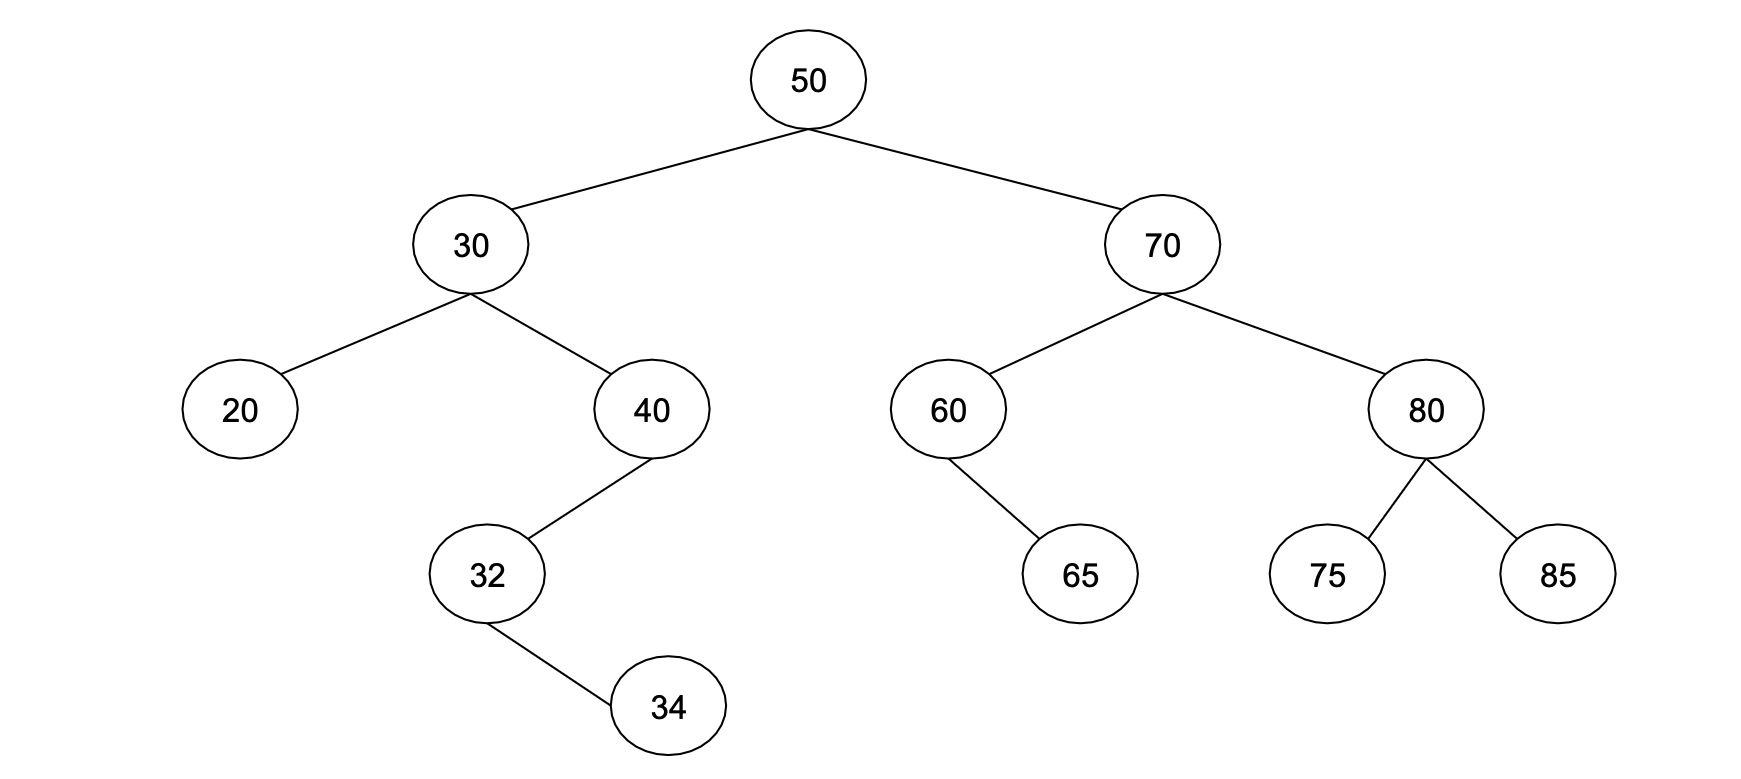
\includegraphics[width=1\textwidth]{images/bst.png}
    \caption{BST di esempio.} % Aggiunge una didascalia
    \label{fig:logo} % Aggiunge un'etichetta per fare riferimento all'immagine
\end{figure}

\begin{itemize}
    \item \textbf{Attraversamento In-Ordine (In-order Traversal)}, complessità: $\Theta(n)$
    \begin{itemize}
        \item \textbf{Descrizione:} Questo algoritmo visita un albero binario di ricerca (BST) processando prima il sottoalbero sinistro, poi la radice e infine il sottoalbero destro. Il risultato è la stampa delle chiavi dei nodi in ordine non decrescente.

        \item \textbf{Esempio:} Dato un albero con le chiavi disposte come nell'esempio del documento, la sequenza di output dell'attraversamento in-ordine è:
        \begin{verbatim}
20, 30, 32, 34, 40, 50, 60, 65, 70, 75, 80, 85
        \end{verbatim}
    \end{itemize}

    \item \textbf{Attraversamento Pre-Ordine (Pre-order Traversal)}, complessità: $\Theta(n)$
    \begin{itemize}
        \item \textbf{Descrizione:} L'attraversamento anticipato (o pre-ordine) visita prima la radice, poi ricorsivamente il sottoalbero sinistro e infine ricorsivamente il sottoalbero destro.

        \item \textbf{Esempio:} Utilizzando lo stesso albero di riferimento, l'output dell'attraversamento pre-ordine è:
        \begin{verbatim}
50, 30, 20, 40, 32, 34, 70, 60, 65, 80, 75, 85
        \end{verbatim}
    \end{itemize}

    \item \textbf{Attraversamento Post-Ordine (Post-order Traversal)}, complessità: $\Theta(n)$
    \begin{itemize}
        \item \textbf{Descrizione:} L'attraversamento posticipato (o post-ordine) visita ricorsivamente prima il sottoalbero sinistro, poi il sottoalbero destro e infine la radice.

        \item \textbf{Esempio:} Per lo stesso albero, la sequenza di output generata è:
        \begin{verbatim}
20, 34, 32, 40, 30, 65, 60, 75, 85, 80, 70, 50
        \end{verbatim}
    \end{itemize}

    \item \textbf{Attraversamento per Livelli (Level-order Traversal)}, complessità: $\Theta(n)$
    \begin{itemize}
        \item \textbf{Descrizione:} Questo algoritmo visita i nodi dell'albero livello per livello, da sinistra a destra, partendo dalla radice. Si avvale di una coda per tenere traccia dei nodi da visitare: la radice viene inserita in coda, e poi, in un ciclo, il nodo in testa alla coda viene rimosso, la sua chiave stampata e i suoi figli (se esistenti) vengono aggiunti alla coda.

        \item \textbf{Esempio:} Per l'albero di riferimento, l'output dell'attraversamento per livelli sarebbe:
        \begin{verbatim}
50, 30, 70, 20, 40, 60, 80, 32, 65, 75, 85, 34
        \end{verbatim}
    \end{itemize}
\end{itemize}